\documentclass[11pt]{amsbook}

\usepackage[turkish]{babel}
\usepackage{../Ceyhun}
\usepackage{../amsTurkish}

\begin{document}
\hPage{014}

\[
	\Omega_8 = (d_2, d_3, d_4, d_6, d_7, d_9)
\]

\[
	\tilde{\Omega}_8 = (d_2, d_3, d_4, d_6, d_7, d_8, d_9)
\]

$\Omega_8$ ve $\tilde{\Omega}_8$ in irgittiği altçizgeler sırasıyla, \\
Şekil \ref{fig:1b} ve \ref{fig:1c}de gösterilmiştir.

\begin{figure}[htbp]

\begin{center}
\subfigure[]{
	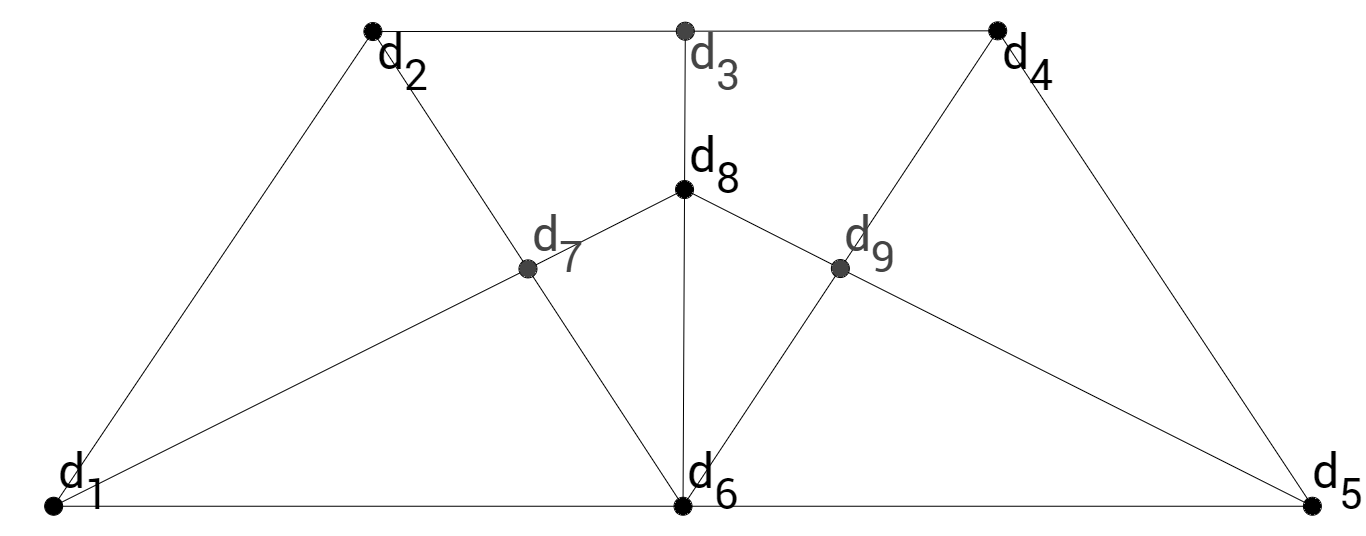
\includegraphics[width=0.5\columnwidth] {images/ceyhun-014-fig01a.png}
	\label{fig:1a}
}

\subfigure[]{
	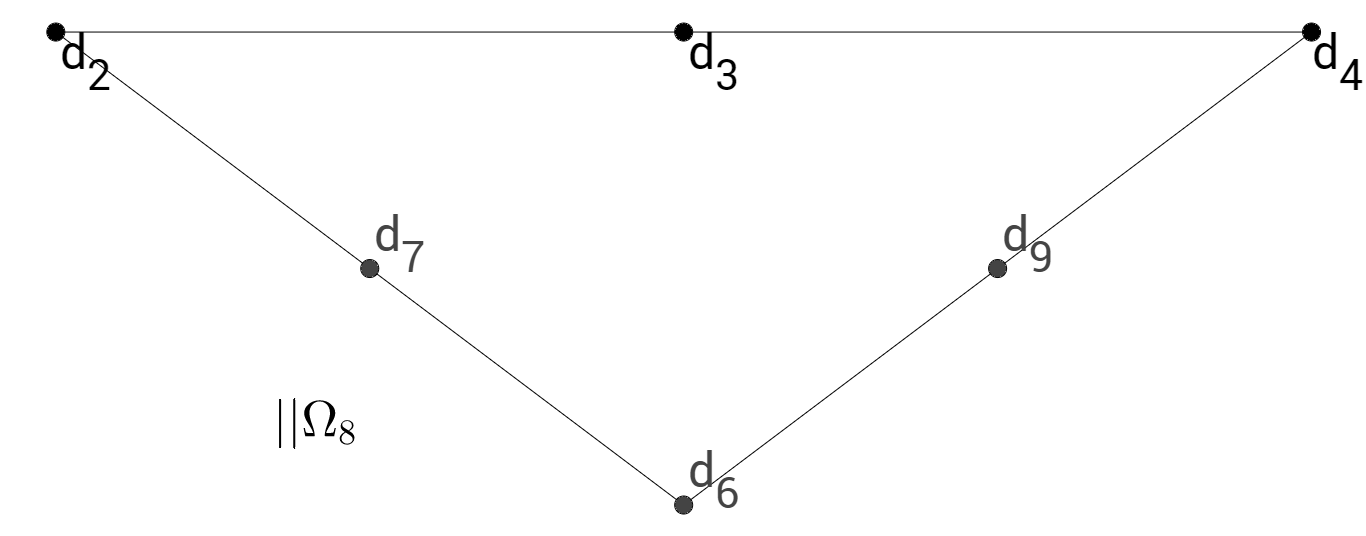
\includegraphics[width=0.5\columnwidth] {images/ceyhun-014-fig01b.png}
	\label{fig:1b}
}

\subfigure[]{
	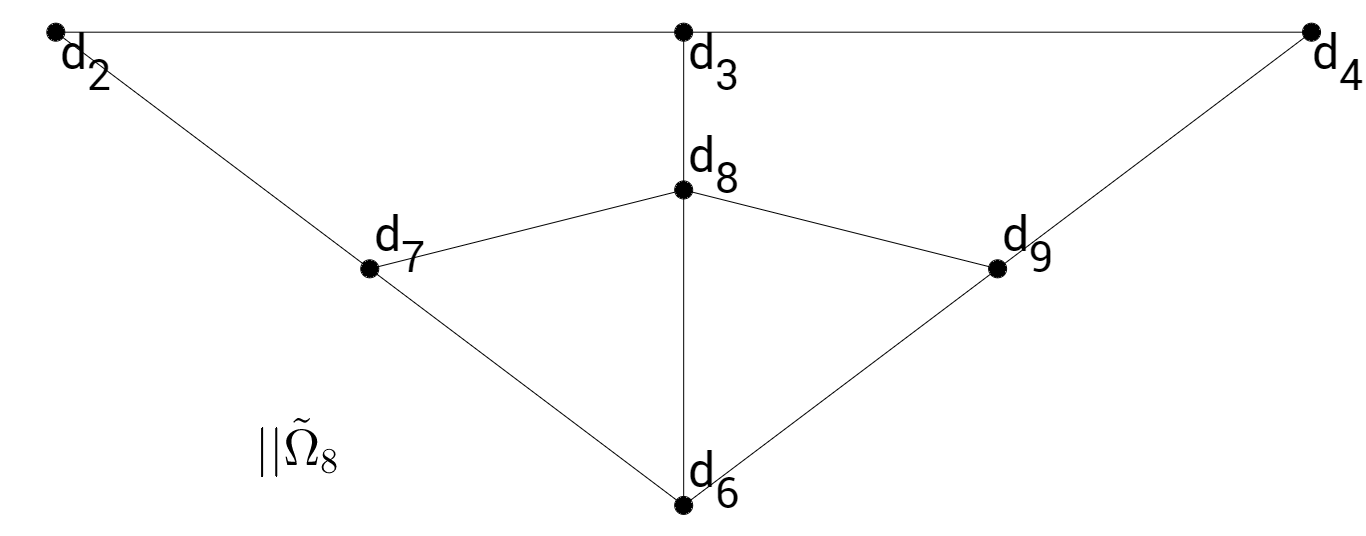
\includegraphics[width=0.5\columnwidth] {images/ceyhun-014-fig01c.png}
	\label{fig:1c}
}

\caption{Yöre ve irgitilmiş altçizgenin açıklanması.}

\end{center}

\end{figure}



\end{document}